Uma instância do sistema modelado foi definida com os seguintes valores sendo atribuídos às variáveis do sistema: $m = 2.35\ kg$, $g = 9,81\ m/s^2$, $l = 0,5\ m$, $I_{xx} = 0.1676\ kg.m^2$, $I_{yy} = 0.1686\ kg.m^2$, $I_{zz} = 0.29743\ kg.m^2$, $\phi_0 = \theta_0 = \psi_0 = 0\ rad$, em que: $m$ é a massa do quadrotor; $g$, a aceleração da gravidade; $l$, a distância de cada rotor ao centro do quadrotor; $I_{xx}$, o momento de inércia ao longo do eixo $x$; $I_{yy}$, o momento de inércia ao longo do eixo $y$; $I_{zz}$, o momento de inércia ao longo do eixo $z$; $\theta$, o ângulo de arfagem; $\phi$, o ângulo de rolamento; e $\psi$, o ângulo de guinada.

\subsection{Funções de Transferência}
\label{subsec:tfs}
%Funções de transferência parcial
Após executar o código do Apêndice \ref{chap:apendicex-quadcopter-modelagem}, a variável {\ttfamily Smoving} armazena as funções de transferência do sistema. Os Quadros \ref{qua:resultados_quadro_tfs_u1}, \ref{qua:resultados_quadro_tfs_u2}, \ref{qua:resultados_quadro_tfs_u3} e \ref{qua:resultados_quadro_tfs_u4} sintetizam os resultados relacionando todas as funções de transferência relacionadas às entradas $u_1$, $u_2$, $u_3$ e $u_4$ respectivamente. Como foi implementado um bloco de desacoplamento das entradas, cada saída é, de fato, influenciada por uma única entrada.

\begin{quadro}[!htb]
    \centering
    \caption{Funções de transferência parciais referentes à entrada $u_1$\label{qua:resultados_quadro_tfs_u1}}
    \begin{tabular}{|c|c|}
    % \begin{tabular}{>{\centering\bfseries}m{1in} >{\centering}m{1in}
        \hline
        \textbf{Saída} & 
        \textbf{Função de Transferência} \\
        \hline
            $z$ &
            $\frac{-0.4249}{s^2}$ \\[1ex]
        \hline
            $\dot{z}$ &
            $\frac{-0.4249}{s}$ \\[1ex]
        \hline
    \end{tabular}
    % \begin{TAB}(r,1cm,2cm)[5pt]{|c|c|}{|c|c|c|}% (rows,min,max)[tabcolsep]{columns}{rows}
    %     hi & tall one    \\
    %     hi & medium one  \\
    %     hi & standard one\\
    % \end{TAB}
\end{quadro}


\begin{quadro}[!htb]
    \centering
    \caption{Funções de transferência parciais referentes à entrada $u_2$\label{qua:resultados_quadro_tfs_u2}}
    \begin{tabular}{|c|c|}
        \hline
        \textbf{Saída} & 
        \textbf{Função de Transferência} \\
        \hline
            $y$ &
            $\frac{58.53}{s^4}$ \\[1ex]
        \hline
            $\dot{y}$ &
            $\frac{58.53}{s^3}$ \\[1ex]
        \hline
            $\phi$ &
            $\frac{5.967}{s^2}$ \\[1ex]
        \hline
            $\dot{\phi}$ &
            $\frac{5.967}{s}$ \\[1ex]
        \hline
    \end{tabular}
\end{quadro}


\begin{quadro}[!htb]
    \centering
    \caption{Funções de transferência parciais referentes à entrada $u_3$\label{qua:resultados_quadro_tfs_u3}}
    \begin{tabular}{|c|c|}
        \hline
        \textbf{Saída} & 
        \textbf{Função de Transferência} \\
        \hline
            $x$ &
            $\frac{-58.19}{s^4}$ \\[1ex]
        \hline
            $\dot{x}$ &
            $\frac{-58.19}{s^3}$ \\[1ex]
        \hline
            $\theta$ &
            $\frac{5.931}{s^2}$ \\[1ex]
        \hline
            $\dot{\theta}$ &
            $\frac{5.931}{s}$ \\[1ex]
        \hline
    \end{tabular}
\end{quadro}


\begin{quadro}[!htb]
    \centering
    \caption{Funções de transferência parciais referentes à entrada $u_4$\label{qua:resultados_quadro_tfs_u4}}
    \begin{tabular}{|c|c|}
        \hline
        \textbf{Saída} & 
        \textbf{Função de Transferência} \\
        \hline
            $\psi$ &
            $\frac{3.362}{s^2}$ \\[1ex]
        \hline
            $\dot{\psi}$ &
            $\frac{3.362}{s}$ \\[1ex]
        \hline
    \end{tabular}
\end{quadro}


% Exibir subbloco criado e sistema construído
A partir destas funções de transferência, foi criado um bloco no Simulink, representando todo o comportamento do quadrotor modelado. As Figuras \ref{fig:resultados-bloco-sistema-drone-geral} e \ref{fig:resultados-bloco-sistema-drone-subsistema} mostram o bloco resultante construído e o subsistema incorporado por ele, respectivamente.

\begin{figure}[!htb]
    \centering
    \caption{Bloco desenvolvido para representar o funcionamento do quadrotor}
    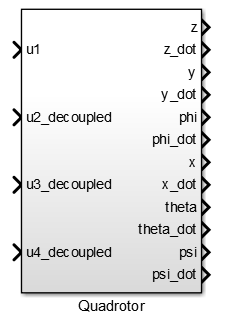
\includegraphics[width=0.3\textwidth]{./04-figuras/resultados/resultados_bloco_quadrotor}
    \label{fig:resultados-bloco-sistema-drone-geral}
\end{figure}

\begin{figure}[!htb]
    \centering
    \caption{Subsistema que compõe o bloco desenvolvido para representar o funcionamento do quadrotor}
    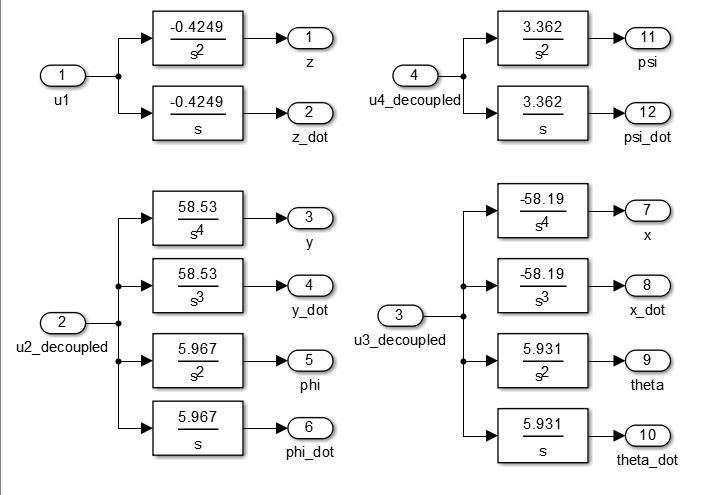
\includegraphics[width=1\textwidth]{./04-figuras/resultados/resultados_bloco_quadrotor_subsistema}
    \label{fig:resultados-bloco-sistema-drone-subsistema}
\end{figure}

\subsection{Análise em Malha Aberta}
\label{subsec:malha_aberta}

Para a análise gráfica da resposta de cada saída a uma excitação em cada entrada, foram utilizados o sistemas mostrados nas Figuras \ref{fig:resultados_bloco_quadrotor_entrada_u1}, \ref{fig:resultados_bloco_quadrotor_entrada_u2}, \ref{fig:resultados_bloco_quadrotor_entrada_u3} e \ref{fig:resultados_bloco_quadrotor_entrada_u4}, que representam o sistema em malha aberta para excitação individual em cada uma de suas quatro entradas. Em todos os casos, a excitação foi definida por um degrau unitário no instante $t=0$.

% Exibir sistema com entrada degrau aplicada à entrada u1
\begin{figure}[!htb]
    \centering
    \caption{Diagrama do sistema simulado para verificar influência da entrada $u_1$ nas saídas}
    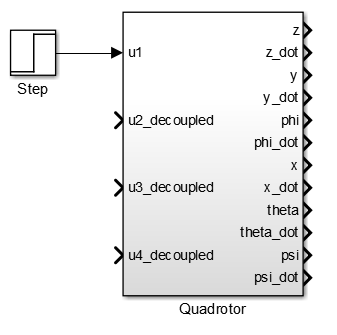
\includegraphics[width=0.3\textwidth]{./04-figuras/resultados/malha_aberta/resultados_bloco_quadrotor_entrada_u1}
    \label{fig:resultados_bloco_quadrotor_entrada_u1}
\end{figure}

% Explicar resultados de u1 em malha aberta
Analisando todas as saídas do sistema mostrado na Figura \ref{fig:resultados_bloco_quadrotor_entrada_u1}, percebeu-se que, com exceção das saídas $z$ e $\dot{z}$, todas as demais ficaram inalteradas. Este resultado já era esperado devido ao bloco de desacoplamento incorporado pelo sistema. As respostas das saídas $z$ e $\dot{z}$ à excitação em degrau unitário sobre a entrada $u_1$ são mostrados na Figura \ref{fig:resultados_malha_aberta_u1_z}. Nota-se que a velocidade ao longo do eixo $z$, definida por $\dot{z}$, se altera linearmente, ao passo que a posição sobre o eixo, definida por $z$ se altera de forma quadrática. Isto indica que o valor aplicado na entrada $u_1$ é, na realidade, a aceleração do quadrotor sobre o eixo z.

% Exibir resposta de todas as saídas referentes em malha aberta para u1
\begin{figure}[!htb]
    \centering
    \caption{Resposta de $z$ e $\dot{z}$ a uma excitação em degrau unitário no tempo $t=0$ na entrada $u_1$}
    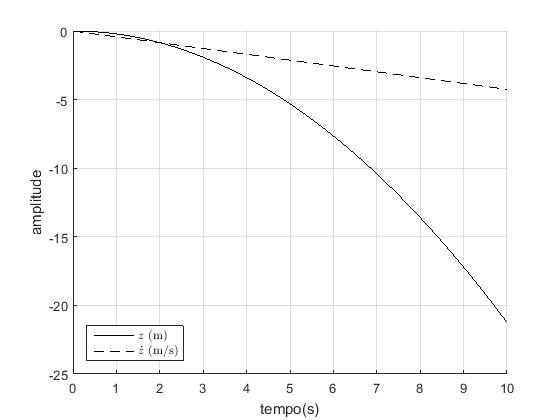
\includegraphics[width=0.8\textwidth]{./04-figuras/resultados/malha_aberta/u1_z}
    \label{fig:resultados_malha_aberta_u1_z}
\end{figure}

O mesmo procedimento foi realizado para verificar a resposta das saídas a uma excitação na entrada $u_2$. Desta vez, verificou-se que somente as saídas $y$, $\dot{y}$, $\phi$ e $\dot{\phi}$ foram alteradas. A Figura \ref{fig:resultados_bloco_quadrotor_entrada_u2} exibe o sistema analisado ao passo que a Figura \ref{fig:resultados_malha_aberta_u2_y} mostra as respostas das saídas $y$ e $\dot{y}$ e a Figura \ref{fig:resultados_malha_aberta_u2_phi} mostra as respostas de $\phi$ e $\dot{\phi}$.

% Exibir sistema com entrada degrau aplicada à entrada u2
\begin{figure}[!htb]
    \centering
    \caption{Diagrama do sistema simulado para verificar influência da entrada $u_2$ nas saídas}
    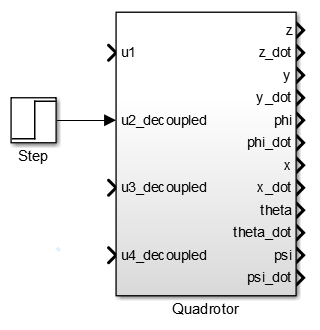
\includegraphics[width=0.3\textwidth]{./04-figuras/resultados/malha_aberta/resultados_bloco_quadrotor_entrada_u2}
    \label{fig:resultados_bloco_quadrotor_entrada_u2}
\end{figure}

% Exibir resposta de todas as saídas referentes em malha aberta para u2 (y)
\begin{figure}[!htb]
    \centering
    \caption{Resposta de $y$ e $\dot{y}$ a uma excitação em degrau unitário no tempo $t=0$ na entrada $u_2$}
    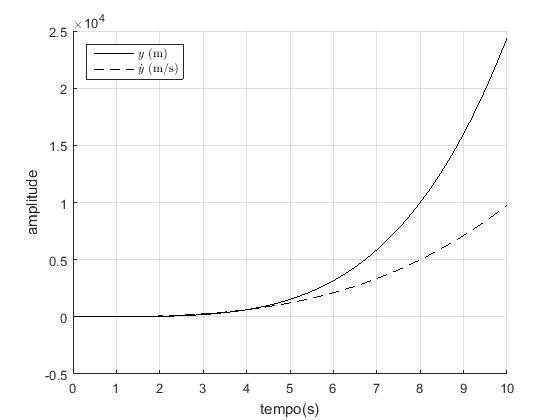
\includegraphics[width=0.8\textwidth]{./04-figuras/resultados/malha_aberta/u2_y}
    \label{fig:resultados_malha_aberta_u2_y}
\end{figure}
% Exibir resposta de todas as saídas referentes em malha aberta para u2 (phi)
\begin{figure}[!htb]
    \centering
    \caption{Resposta de $\phi$ e $\dot{\phi}$ a uma excitação em degrau unitário no tempo $t=0$ na entrada $u_2$}
    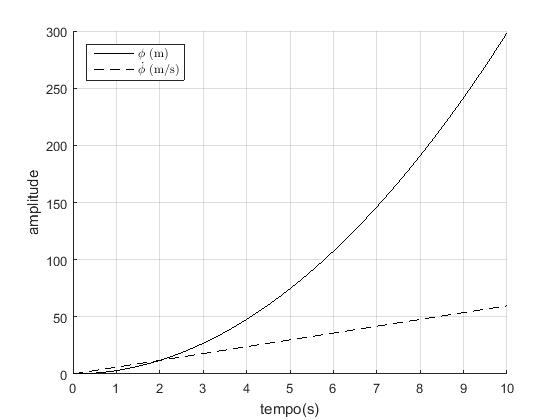
\includegraphics[width=0.8\textwidth]{./04-figuras/resultados/malha_aberta/u2_phi}
    \label{fig:resultados_malha_aberta_u2_phi}
\end{figure}

% Explicar resultados de u2 em malha aberta
Assim como ocorreu com as saídas $z$ e $\dot{z}$, nota-se que o ângulo em torno do eixo y, $\phi$, cresce de forma linear ao passo que a velocidade angular em torno deste mesmo eixo, $\dot{\phi}$, cresce de forma quadrática. Já as saídas $y$ e $\dot{y}$, posição sobre o eixo y velocidade sobre este eixo, respectivamente, variam ambas de forma polinomial, com $y$ apresentando maior grau se comparado a $\dot{y}$. Este resultado era o esperado, tendo em vista que um crescimento na velocidade (aceleração positiva) leva a uma maior taxa de variação da posição. Analogamente ao resultado obtido sobre a entrada $u_1$, nota-se que a entrada $u_2$ representa a aceleração angular sobre o eixo x.

A próxima entrada a ser analisada foi a $u_3$. A Figura \ref{fig:resultados_bloco_quadrotor_entrada_u3} mostra o sistema utilizado. Desta vez, assim como era esperado devido ao desacoplamento das entradas, somente as saídas $x$, $\dot{x}$, $\theta$ e $\dot{\theta}$ foram influenciadas. A Figura \ref{fig:resultados_malha_aberta_u3_x} mostra a resposta de $x$ e $\dot{x}$ enquanto a Figura \ref{fig:resultados_malha_aberta_u3_theta} mostra a resposta das saídas $\theta$ e $\dot{\theta}$.

% Exibir sistema com entrada degrau aplicada à entrada u3
\begin{figure}[!htb]
    \centering
    \caption{Diagrama do sistema simulado para verificar influência da entrada $u_3$ nas saídas}
    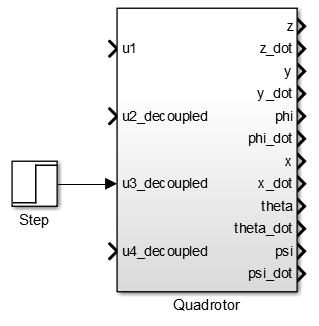
\includegraphics[width=0.3\textwidth]{./04-figuras/resultados/malha_aberta/resultados_bloco_quadrotor_entrada_u3}
    \label{fig:resultados_bloco_quadrotor_entrada_u3}
\end{figure}

% Exibir resposta de todas as saídas referentes em malha aberta para u3 (x)
\begin{figure}[!htb]
    \centering
    \caption{Resposta de $x$ e $\dot{x}$ a uma excitação em degrau unitário no tempo $t=0$ na entrada $u_3$}
    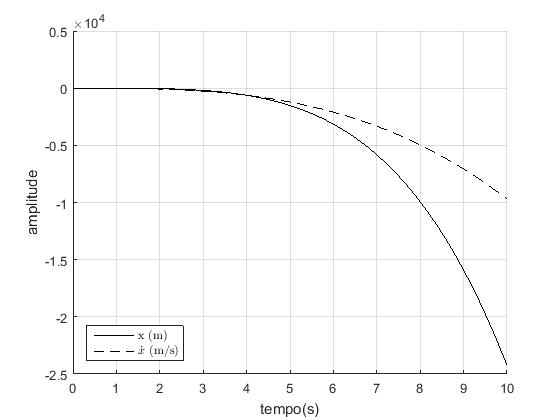
\includegraphics[width=0.8\textwidth]{./04-figuras/resultados/malha_aberta/u3_x}
    \label{fig:resultados_malha_aberta_u3_x}
\end{figure}
% Exibir resposta de todas as saídas referentes em malha aberta para u3 (theta)
\begin{figure}[!htb]
    \centering
    \caption{Resposta de $\theta$ e $\dot{\theta}$ a uma excitação em degrau unitário no tempo $t=0$ na entrada $u_3$}
    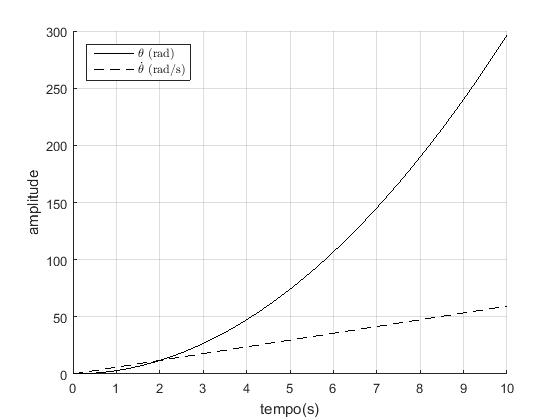
\includegraphics[width=0.8\textwidth]{./04-figuras/resultados/malha_aberta/u3_theta}
    \label{fig:resultados_malha_aberta_u3_theta}
\end{figure}

% Explicar resultados de u3 em malha aberta
Nota-se que o comportamento do sistema ao degrau unitário em $u_3$ é bastante similar ao obtido quando a entrada excitada foi a $u_2$. Isto já era esperado tendo em vista que as funções de transferência que relacionam as saídas a estas duas entradas são bastante próximas. A única diferença observada é o fato de a posição sobre o eixo x decrescer, enquanto a posição sobre o eixo y era incrementada. Isto ocorre pelo fato de \citeonline{Balas2007} ter definido, durante a modelagem do quadrotor, que para caminhar no eixo positivo do eixo x, o ângulo $\theta$ deveria receber um valor negativo e vice-versa.

Assim como se percebeu ao analisar a resposta do sistema à entrada $u_2$, percebe-se que a entrada $u_3$ representa a aceleração angular do drone sobre o eixo y.

Por fim, analisou-se o comportamento do sistema quando uma entrada em degrau unitário é aplicado sobre a entrada $u_4$. A Figura \ref{fig:resultados_bloco_quadrotor_entrada_u4} mostra o sistema simulado e a Figura \ref{fig:resultados_malha_aberta_u4_psi} mostra o comportamento das saídas afetadas por esta excitação.

% Exibir sistema com entrada degrau aplicada à entrada u4
\begin{figure}[!htb]
    \centering
    \caption{Diagrama do sistema simulado para verificar influência da entrada $u_4$ nas saídas}
    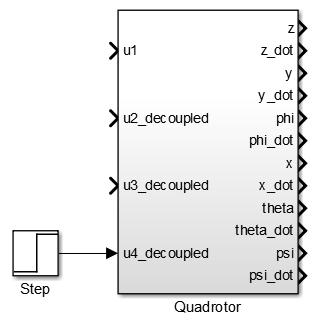
\includegraphics[width=0.3\textwidth]{./04-figuras/resultados/malha_aberta/resultados_bloco_quadrotor_entrada_u4}
    \label{fig:resultados_bloco_quadrotor_entrada_u4}
\end{figure}

% Exibir resposta de todas as saídas referentes em malha aberta para u4 (psi)
\begin{figure}[!htb]
    \centering
    \caption{Resposta de $\psi$ e $\dot{\psi}$ a uma excitação em degrau unitário no tempo $t=0$ na entrada $u_4$}
    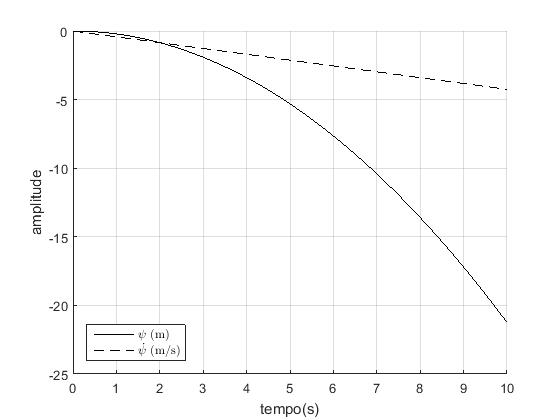
\includegraphics[width=0.8\textwidth]{./04-figuras/resultados/malha_aberta/u4_psi}
    \label{fig:resultados_malha_aberta_u4_psi}
\end{figure}

Somente as saídas $\psi$ e $\dot{psi}$ sofreram alteração. Como se pode ver, a saída $\dot{\psi}$, referente à velocidade angular sobre o eixo z, decresce linearmente, enquanto $\psi$, o ângulo em torno do eixo decresce quadraticamente. Assim como nos outros casos observados, a entrada $u_4$ é a aceleração para uma variável do sistema: desta vez, é a aceleração angular em torno do eixo z.

\subsection{Controle de Atitude}
\label{subsec:controle_atitude}

Para permitir que o quadrotor se comporte de forma estável, foi feito o controle isoladamente dos dois eixos que formam o plano horizontal do sistema: x e y. Em ambos os casos, a função do controlador é fazer com que, após perturbado, o quadrotor volte a se estabilizar horizontalmente, ou seja, volte ao estado em que $\theta$ e $\phi$ sejam zero. Devido à simetria existente entre os eixos x e y, um mesmo controlador pôde ser utilizado para controlar o ângulo do drone em torno de ambos os eixos.

A Figura \ref{fig:u2_mamdani_blocks} mostra o diagrama do sistema de controle Fuzzy sobre a entrada $u_2$ e a Figura \ref{fig:u3_mamdani_blocks} sobre a entrada $u_3$. Nota-se que uma entrada de ruído foi inserida nos sistemas. Esta entrada oferece uma perturbação momentânea ao sistema. Este sinal de ruído como sendo um degrau de amplitude 20 e duração de quatro centésimos de segundo, para representar uma aceleração intensa mas quase instantânea. O papel do controlador é fazer com que, mesmo após esta perturbação, o quadrotor volte à estabilidade angular.

% Mostrar diagrama do sistema controlado (para ruídos), sobre as entradas u2 e u3
\begin{figure}[!htb]
    \centering
    \caption{Diagrama do sistema de controle Fuzzy Mamdani sobre o ângulo $\phi$}
    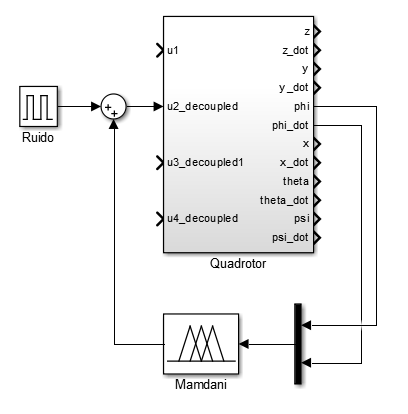
\includegraphics[width=0.5\textwidth]{./04-figuras/resultados/fis_u2/u2_mamdani_blocks}
    \label{fig:u2_mamdani_blocks}
\end{figure}

\begin{figure}[!htb]
    \centering
    \caption{Diagrama do sistema de controle Fuzzy Mamdani sobre o ângulo $\theta$}
    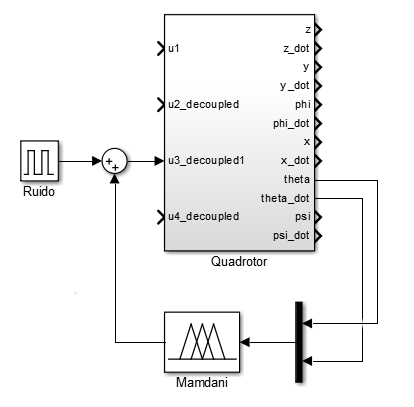
\includegraphics[width=0.5\textwidth]{./04-figuras/resultados/fis_u3/u3_mamdani_blocks}
    \label{fig:u3_mamdani_blocks}
\end{figure}

Como se pode ver pela figura, o controlador desenvolvido inicialmente foi do tipo Fuzzy Mamdani. As entradas do controlador referentes à ao eixo y são $\phi$ e $\dot{\phi}$, e a saída é o sinal de controle para o $u_2$. Já as entradas do controlador do eixo x são $\theta$ e $\dot{\theta}$ e a saída é o sinal de controle para $u_3$. Tanto as entradas quanto a saída foram divididas em três grupos, cada qual referente a uma função de pertinência: N (negativo), Z (zero) e P (positivo). Todas estas funções são do tipo triangular. O Quadro \ref{qua:regras_fuzzy_u2_u3_mamdani} sintetiza as regras utilizadas pelo controlador.

% Mostrar regras Fuzzy envolvidas no controle de u2 e u3 (quadro de regras + superfície)
\begin{quadro}[!htb]
    \centering
    \caption{Regras fuzzy para modelagem do controle de atitude\label{qua:regras_fuzzy_u2_u3_mamdani}}
    \begin{tabular}{|c|c|c|}
    % \begin{tabular}{>{\centering\bfseries}m{1in} >{\centering}m{1in}
        \hline
        \textbf{{$\phi/\theta$}} & 
        \textbf{{$\dot{\phi}/\dot{\theta}$}} &
        \textbf{{$u_2/u_3$}} \\
        \hline %01
            P &
            P &
            N \\
        \hline %02
            P &
            Z &
            N \\
        \hline %03
            P &
            N &
            Z \\
        \hline %04
            N &
            N &
            P \\
        \hline %05
            N &
            Z &
            P \\
        \hline %06
            N &
            P &
            Z \\
        \hline %07
            Z &
            Z &
            Z \\
        \hline %08
            Z &
            N &
            P \\
        \hline %09
            Z &
            P &
            N \\
        \hline
    \end{tabular}
    % \begin{TAB}(r,1cm,2cm)[5pt]{|c|c|}{|c|c|c|}% (rows,min,max)[tabcolsep]{columns}{rows}
    %     hi & tall one    \\
    %     hi & medium one  \\
    %     hi & standard one\\
    % \end{TAB}
\end{quadro}


Uma forma gráfica de se visualizarem as regras é a partir da superfície mostrada na Figura \ref{fig:u2_u3_mamdani_surface}.

\begin{figure}[!htb]
    \centering
    \caption{Superfície das regras do sistema de controle Fuzzy Mamdani para a atitude do quadrotor}
    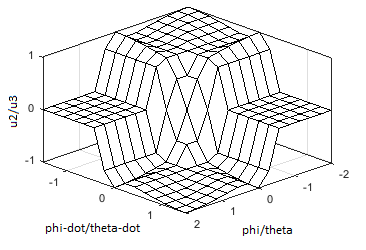
\includegraphics[width=0.6\textwidth]{./04-figuras/resultados/fis_u2/u2_u3_mamdani_surface}
    \label{fig:u2_u3_mamdani_surface}
\end{figure}

A Figura \ref{fig:u2_mamdani_u2_phi} mostra a resposta das saídas $\phi$ e $\dot{\phi}$ à excitação de ruído na entrada $u_2$ do sistema controlado. Como se pode ver, o sistema converge e o ângulo $\phi$, assim como a velocidade angular $\dot{\phi}$, voltam a um valor muito próximo de zero. A Figura \ref{fig:u2_mamdani_u2_phi_regime_permanente} mostra, entretanto, que o valor não volta de fato a zero, apesar de aproximar bastante disso.

% Mostrar resultados obtidos com controle de u2
\begin{figure}[!htb]
    \centering
    \caption{Resposta das saídas $\phi$ e $\dot{\phi}$ no sistema controlado do tipo Mamdani submetido a ruído na entrada $u_2$}
    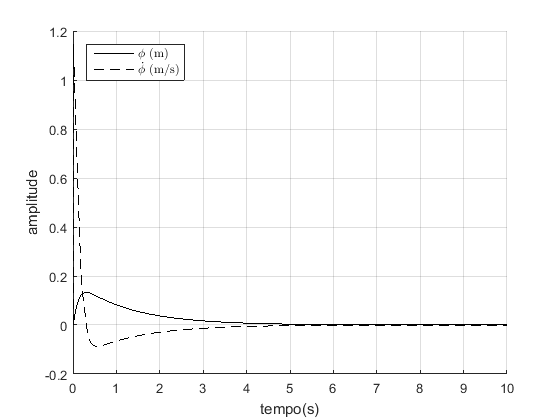
\includegraphics[width=0.8\textwidth]{./04-figuras/resultados/fis_u2/u2_mamdani_u2_phi}
    \label{fig:u2_mamdani_u2_phi}
\end{figure}

\begin{figure}[!htb]
    \centering
    \caption{Resposta das saídas $\phi$ e $\dot{\phi}$ em regime permanente do sistema controlado do tipo Mamdani para perturbação na entrada $u_2$}
    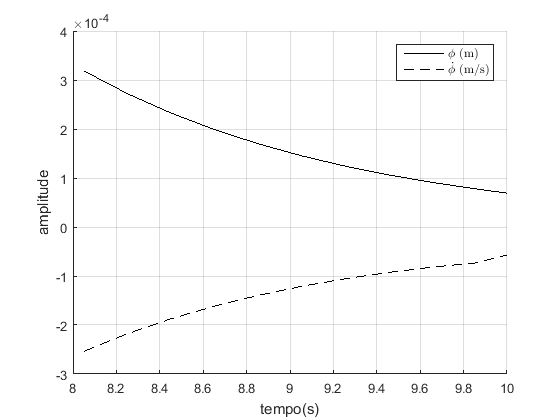
\includegraphics[width=0.8\textwidth]{./04-figuras/resultados/fis_u2/u2_mamdani_u2_phi_regime_permanente}
    \label{fig:u2_mamdani_u2_phi_regime_permanente}
\end{figure}

De forma similar, a Figura \ref{fig:u3_mamdani_u3_theta} mostra a resposta das saídas $\theta$ e $\dot{\theta}$ à excitação de ruído na entrada $u_3$ do sistema controlado. Assim como ocorreu no controle do ângulo sobre o eixo y, o ângulo $\theta$ e a velocidade angular $\dot{\theta}$, ambos em torno do eixo x, convergem para um valor muito próximo de zero. A Figura \ref{fig:u3_mamdani_u3_theta_regime_permanente}, entretanto, mostra que o valor de convergência tende a zero, mas não o alcança.

% Mostrar resultados obtidos com controle de u3
\begin{figure}[!htb]
    \centering
    \caption{Resposta das saídas $\theta$ e $\dot{\theta}$ no sistema controlado do tipo Mamdani submetido a ruído na entrada $u_3$}
    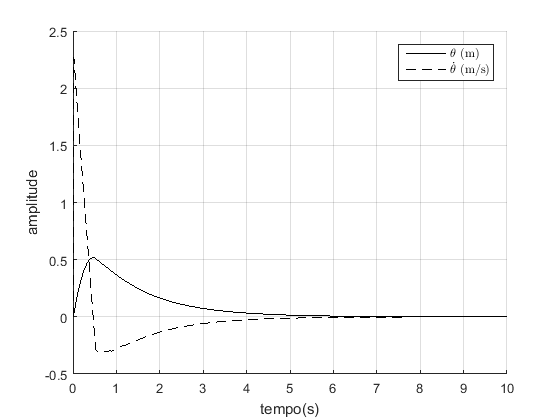
\includegraphics[width=0.8\textwidth]{./04-figuras/resultados/fis_u3/u3_mamdani_u3_theta}
    \label{fig:u3_mamdani_u3_theta}
\end{figure}

\begin{figure}[!htb]
    \centering
    \caption{Resposta das saídas $\theta$ e $\dot{\theta}$ em regime permanente do sistema controlado do tipo Mamdani para perturbação na entrada $u_3$}
    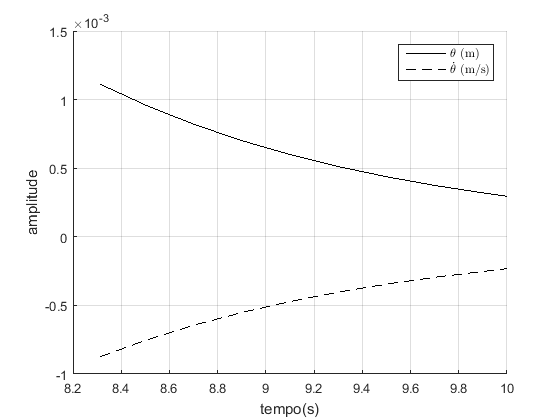
\includegraphics[width=0.8\textwidth]{./04-figuras/resultados/fis_u3/u3_mamdani_u3_theta_regime_permanente}
    \label{fig:u3_mamdani_u3_theta_regime_permanente}
\end{figure}

% Contextualizar criação do neuro-fuzzy
A partir do controlador Fuzzy para atitude, foi construído um controlador Neuro-Fuzzy que, pelo fato de agregar a aprendizagem inteligente e a capacidade de generalização, acreditou-se que poderia melhorar os resultados obtidos pelo controlador Fuzzy, bem como aumentar sua robustez.

% Explicar processo de treinamento
Primeiramente, obteve-se um controlador Fuzzy Sugeno equivalente ao Mamdani previamente construído e, então, foram utilizados resultados do próprio Mamdani para treinar a rede Neuro-Fuzzy, ou seja, para ajustar os parâmetros do Controlador Sugeno. Neste processo, foram utilizados duzentos valores para o treinamento e outros cem para o teste da rede.

% Mostrar tabela com pesos

% Mostrar superfície
Após o treinamento, obteve-se superfície de regras para o controlador Neuro-Fuzzy mostrada na Figura \ref{fig:u2_u3_sugeno_surface}.

\begin{figure}[!htb]
    \centering
    \caption{Superfície das regras do sistema de controle Fuzzy Sugeno para a atitude do quadrotor}
    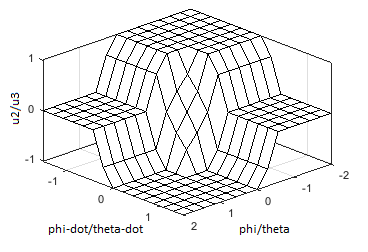
\includegraphics[width=0.6\textwidth]{./04-figuras/resultados/fis_u3/u2_u3_sugeno_surface}
    \label{fig:u2_u3_sugeno_surface}
\end{figure}

% Mostrar blocos com sugeno
O controlador Fuzzy Mamdani foi então substituído pelo Neuro-Fuzzy. Os sistemas de controle Neuro-Fuzzy sobre os ângulos $\phi$ e $\theta$ são mostrados nas Figuras \ref{fig:u2_sugeno_blocks} e \ref{fig:u3_sugeno_blocks} respectivamente.

\begin{figure}[!htb]
    \centering
    \caption{Diagrama do sistema de controle Fuzzy Sugeno sobre o ângulo $\phi$}
    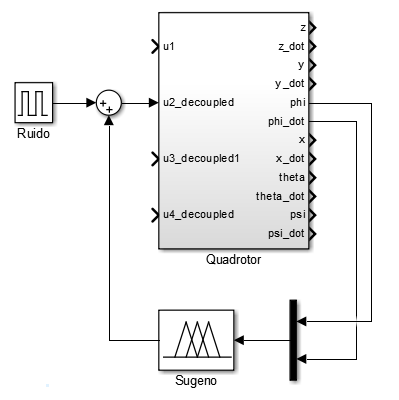
\includegraphics[width=0.5\textwidth]{./04-figuras/resultados/fis_u2/u2_sugeno_blocks}
    \label{fig:u2_sugeno_blocks}
\end{figure}

\begin{figure}[!htb]
    \centering
    \caption{Diagrama do sistema de controle Fuzzy Sugeno sobre o ângulo $\theta$}
    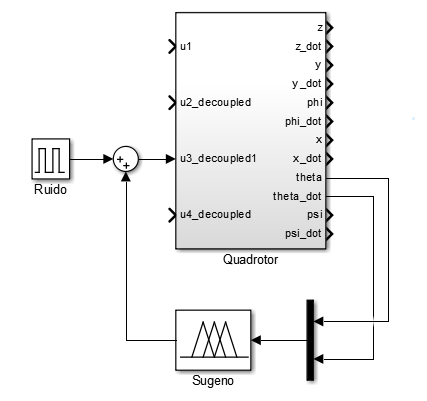
\includegraphics[width=0.5\textwidth]{./04-figuras/resultados/fis_u3/u3_sugeno_blocks}
    \label{fig:u3_sugeno_blocks}
\end{figure}

% Mostrar resultados para u2 e u3

% Mostrar resultados obtidos com controle de u2
\begin{figure}[!htb]
    \centering
    \caption{Resposta das saídas $\phi$ e $\dot{\phi}$ no sistema controlado do tipo Sugeno submetido a ruído na entrada $u_2$}
    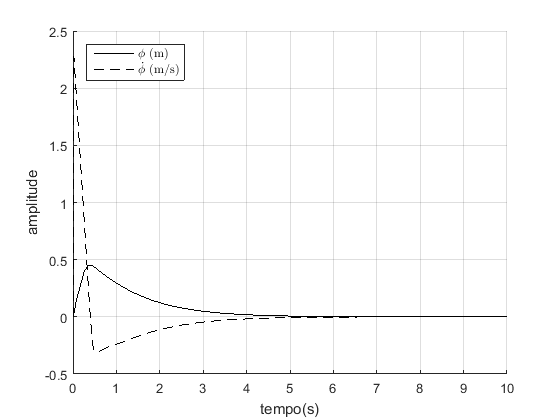
\includegraphics[width=0.8\textwidth]{./04-figuras/resultados/fis_u2/u2_sugeno_u2_phi}
    \label{fig:u2_sugeno_u2_phi}
\end{figure}

\begin{figure}[!htb]
    \centering
    \caption{Resposta das saídas $\phi$ e $\dot{\phi}$ em regime permanente do sistema controlado do tipo Sugeno para perturbação na entrada $u_2$}
    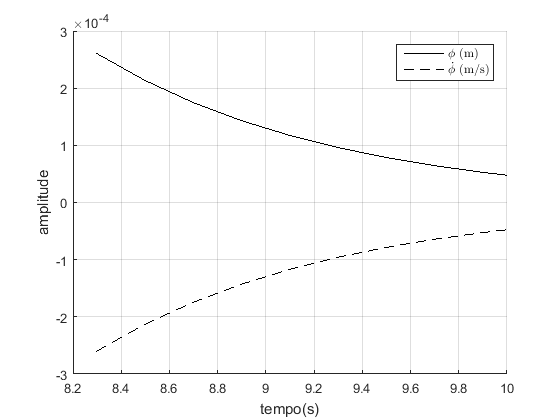
\includegraphics[width=0.8\textwidth]{./04-figuras/resultados/fis_u2/u2_sugeno_u2_phi_regime_permanente}
    \label{fig:u2_sugeno_u2_phi_regime_permanente}
\end{figure}

% Mostrar resultados obtidos com controle de u3
\begin{figure}[!htb]
    \centering
    \caption{Resposta das saídas $\theta$ e $\dot{\theta}$ no sistema controlado do tipo Sugeno submetido a ruído na entrada $u_3$}
    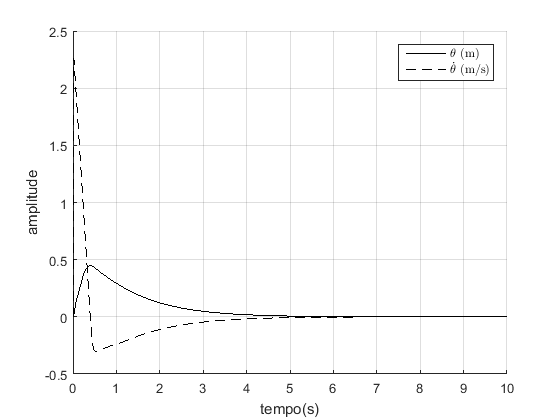
\includegraphics[width=0.8\textwidth]{./04-figuras/resultados/fis_u3/u3_sugeno_u3_theta}
    \label{fig:u3_sugeno_u3_theta}
\end{figure}

\begin{figure}[!htb]
    \centering
    \caption{Resposta das saídas $\theta$ e $\dot{\theta}$ em regime permanente do sistema controlado do tipo Sugeno para perturbação na entrada $u_3$}
    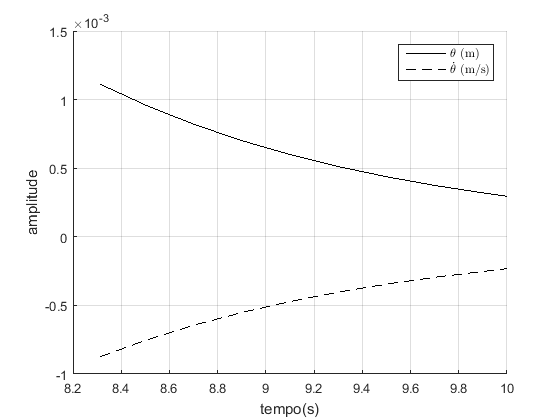
\includegraphics[width=0.8\textwidth]{./04-figuras/resultados/fis_u3/u3_mamdani_u3_theta_regime_permanente}
    \label{fig:u3_sugeno_u3_theta_regime_permanente}
\end{figure}

% Comparar resultados
Comparando as Figuras \ref{fig:u2_mamdani_u2_phi} (Mamdani) e \ref{fig:u2_sugeno_u2_phi} (Sugeno), nota-se que o controlador Neuro-Fuzzy na verdade não ofereceu nenhuma melhora no controle da estabilização do ângulo $\phi$. Ele na verdade aumentou a sobrelevação em mais que 100\% e pouco interferiu no tempo de assetamento.

Por outro lado, comparando as Figuras \ref{fig:u2_mamdani_u2_phi} (Mamdani) e \ref{fig:u2_sugeno_u2_phi} (Sugeno), percebe-se que o controlador Neuro-Fuzzy leva a melhoras sutis no sistema de controle do ângulo $\theta$. Neste caso, ele conseguiu reduzir a sobrelevação do sistema e reduziu levemente o tempo de assentamento.

As leves diferenças entre os sistemas que modelam o eixo x e y do quadrotor foram suficientes para fazer com que um mesmo controlador atue de forma levemente positiva sobre um deles e levemente negativa sobre o outro.

\subsection{Controle de Altitude}
\label{subsec:controle_altitude}

Além do controle de atitude\footnote{Estabilidade angular no plano XY} do drone, efetuou-se também o controle sobre a altitude dele, ou seja, quando sujeito a um distúrbio que o faça oscilar em altitude, ele deveria ser capaz de retomar à posição que ocupava imediatamente antes deste distúrbio.

O procedimento feito para este controle foi similar ao mostrado para o controle de atitude.

A Figura \ref{fig:u1_mamdani_blocks} mostra o diagrama do sistema sujeitado a um distúrbio sobre a entrada $u_1$, que é a única que influencia as saídas $z$ e $\dot{z}$, e já incluindo um controlador Fuzzy do tipo Mamdani. As entradas do controlador são a altitude do drone definida por $z$ e a velocidade neste eixo, $\dot{z}$.

% Mostrar diagrama do sistema controlado (para ruídos), sobre a entrada u1
\begin{figure}[!htb]
    \centering
    \caption{Diagrama do sistema de controle Fuzzy Mamdani sobre a altitude z}
    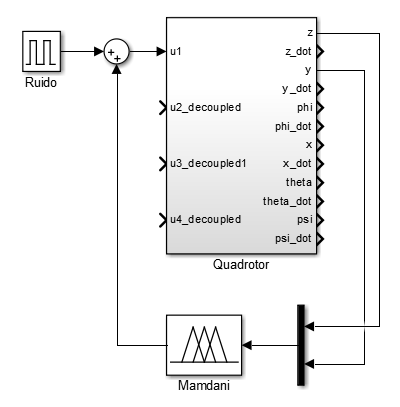
\includegraphics[width=0.5\textwidth]{./04-figuras/resultados/fis_u1/u1_mamdani_blocks}
    \label{fig:u1_mamdani_blocks}
\end{figure}

O Quadro \ref{qua:regras_fuzzy_u1_mamdani} mostra as regras definidas para o controle Fuzzy e a Figura \ref{fig:1_mamdani_surface} exibe a superfície de regras equivalente.

% Mostrar regras Fuzzy envolvidas no controle de u1 (quadro de regras + superfície)
\begin{quadro}[!htb]
    \centering
    \caption{Regras fuzzy para modelagem do controle de altitude\label{qua:regras_fuzzy_u1_mamdani}}
    \begin{tabular}{|c|c|c|}
    % \begin{tabular}{>{\centering\bfseries}m{1in} >{\centering}m{1in}
        \hline
        \textbf{{$z$}} & 
        \textbf{{$\dot{z}$}} &
        \textbf{{$u_1$}} \\
        \hline %01
            N &
            - &
            N \\
        \hline %02
            P &
            - &
            P \\
        \hline %03
            Z &
            N &
            N \\
        \hline %04
            Z &
            Z &
            Z \\
        \hline %05
            Z &
            P &
            P \\
        \hline
    \end{tabular}
    % \begin{TAB}(r,1cm,2cm)[5pt]{|c|c|}{|c|c|c|}% (rows,min,max)[tabcolsep]{columns}{rows}
    %     hi & tall one    \\
    %     hi & medium one  \\
    %     hi & standard one\\
    % \end{TAB}
\end{quadro}


\begin{figure}[!htb]
    \centering
    \caption{Superfície das regras do sistema de controle Fuzzy Mamdani para a altitude do quadrotor}
    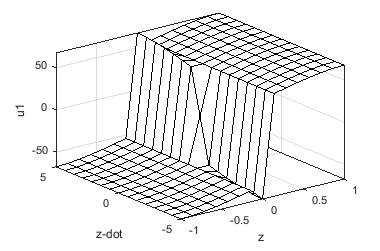
\includegraphics[width=0.6\textwidth]{./04-figuras/resultados/fis_u1/u1_mamdani_surface}
    \label{fig:1_mamdani_surface}
\end{figure}

A Figura \ref{fig:u1_mamdani_z} exibe a saída do sistema definido para controle de altitude. Como se pode ver, logo após o distúrbio, o drone alcança uma velocidade crescente negativa. Desta forma, o controlador age compensando esta velocidade para que ele possa voltar a se estabilizar na altitude que tinha inicialmente, representada por $z=0$. Como se pode ver pela Figura \ref{fig:u1_mamdani_z_regime_permanente}, a altitude $z$ nem a velocidade $\dot{z}$ voltam a ser, de fato, zero, mas ambas se aproximam bastante disso para se considerar que o drone voltou de fato à posição que assumia antes do distúrbio.

% Mostrar resultados obtidos com controle de u1
\begin{figure}[!htb]
    \centering
    \caption{Resposta das saídas $z$ e $\dot{z}$ no sistema controlado do tipo Mamdani submetido a ruído na entrada $u_1$}
    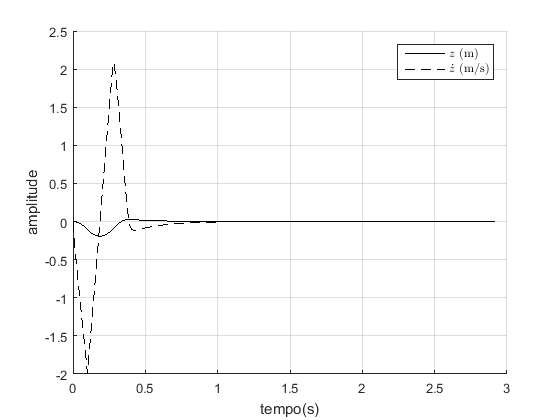
\includegraphics[width=0.8\textwidth]{./04-figuras/resultados/fis_u1/u1_mamdani_z}
    \label{fig:u1_mamdani_z}
\end{figure}

\begin{figure}[!htb]
    \centering
    \caption{Resposta das saídas $z$ e $\dot{z}$ em regime permanente do sistema controlado do tipo Mamdani para perturbação na entrada $u_1$}
    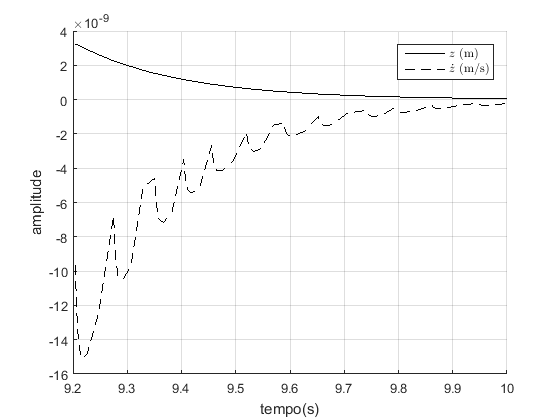
\includegraphics[width=0.8\textwidth]{./04-figuras/resultados/fis_u1/u1_mamdani_z_regime_permanente}
    \label{fig:u1_mamdani_z_regime_permanente}
\end{figure}

Assim como foi feito para o controle de atitude, para o controle de altitude também foi gerado um sistema Neuro-Fuzzy a partir do Fuzzy Mamdani originalmente criado.

Após o treinamento em processo também similar ao de controle de atitude, e mais uma vez mantendo-se as regras de origem, obteve-se a superfície de regras mostrada na Figura \ref{fig:u1_sugeno_surface}.

% Mostrar superfície Sugeno
\begin{figure}[!htb]
    \centering
    \caption{Superfície das regras do sistema de controle Fuzzy Sugeno para a altitude do quadrotor}
    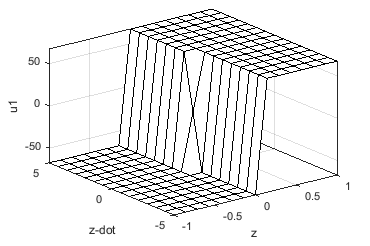
\includegraphics[width=0.6\textwidth]{./04-figuras/resultados/fis_u1/u1_sugeno_surface}
    \label{fig:u1_sugeno_surface}
\end{figure}

% Mostrar blocos com sugeno
O diagrama de blocos mostrando o sistema de controle incorporando o controlador Neuro-Fuzzy é mostrado na Figura 

\begin{figure}[!htb]
    \centering
    \caption{Diagrama do sistema de controle Fuzzy Sugeno sobre a altitude $z$}
    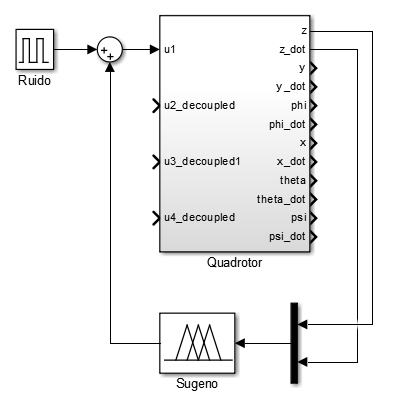
\includegraphics[width=0.5\textwidth]{./04-figuras/resultados/fis_u1/u1_sugeno_blocks}
    \label{fig:u1_sugeno_blocks}
\end{figure}

A resposta deste sistema é mostrado nas Figuras \ref{fig:u1_sugeno_z} e \ref{fig:u1_sugeno_z_regime_permanente}. Como se pode ver ao comparar as Figuras \ref{fig:u1_mamdani_z} e \ref{fig:u1_sugeno_z}, o controlador Neuro-Fuzzy reduziu a sobrelevação tanto de $z$ quanto de $\dot{z}$ além de reduzir também ligeiramente o tempo necessário para $z$ se estabilizar. Comparando as Figuras \ref{fig:u1_mamdani_z_regime_permanente} e \ref{fig:u1_sugeno_z_regime_permanente} percebe-se que o comportamento do sistema submetido aos diferentes controladores difere basante em regime permanente. No caso do controlador Mamdani, há uma variação constante de crescimento e decrescimento da velocidade $\dot{z}$. Já no caso do controlador Sugeno, as variações são menos constantes e possuem maior amplitude.

% Mostrar resultados obtidos com controle de u1
\begin{figure}[!htb]
    \centering
    \caption{Resposta das saídas $z$ e $\dot{z}$ no sistema controlado do tipo Sugeno submetido a ruído na entrada $u_1$}
    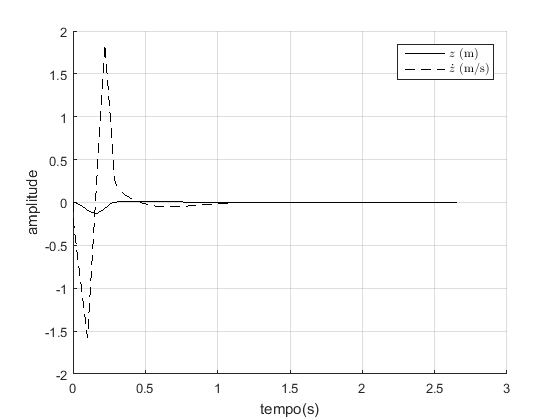
\includegraphics[width=0.8\textwidth]{./04-figuras/resultados/fis_u1/u1_sugeno_z}
    \label{fig:u1_sugeno_z}
\end{figure}

\begin{figure}[!htb]
    \centering
    \caption{Resposta das saídas $z$ e $\dot{z}$ em regime permanente no sistema controlado do tipo Sugeno submetido a ruído na entrada $u_1$}
    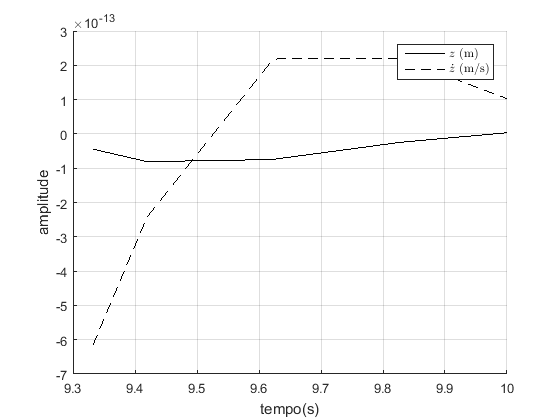
\includegraphics[width=0.8\textwidth]{./04-figuras/resultados/fis_u1/u1_sugeno_z_regime_permanente}
    \label{fig:u1_sugeno_z_regime_permanente}
\end{figure}






% Controle de Altitude

% Mostrar diagrama do sistema controlado (para ruídos), sobre a entrada u1

% Mostrar regras Fuzzy envolvidas no controle de u1 (funções de pertinência + quadro de regras + superfície)

% Mostrar resultados obtidos com controle de u4





